\chapter{Conception}
\section{Purpose of the chapter}
The purpose of this chapter is to present the conception of a virtual counter system for the Algerian National Social Security Fund (CNAS). This chapter will provide a detailed explanation of the system design and architecture, database design, as well as the different diagrams and models used during the conception phase. The virtual counter system aims to improve the current management system used by CNAS by providing users with a more efficient and user-friendly way to gather necessary information and book appointments.
\section {Overview of the topics covered}
This chapter focuses on the conception of the virtual counter system for CNAS. It includes the analysis and design of the system, from the identification of user requirements to the development of the system architecture and database design. The chapter also includes the presentation of the different diagrams that were created, such as the use case diagram, class diagram, sequence diagram, and flowchart.
The aim of this chapter is to provide a comprehensive understanding of the virtual counter system, its components, and its functionalities.

\section{System design and architecture}
The system design and architecture of a virtual counter is a crucial aspect in developing a successful web application. It involves designing the components of the system and specifying how they interact with each other to achieve the desired functionality. In the case of a virtual counter for CNAS, the system design and architecture must take into account the different types of users, such as clients and agents, and the various tasks they need to perform. It must also ensure that the application is secure and reliable, with measures in place to protect user data and prevent unauthorized access. The system design and architecture will involve selecting suitable technologies and frameworks, such as Laravel and VueJs, and designing a database schema to store and retrieve data efficiently. Overall, a well-designed system architecture will contribute to the effectiveness and efficiency of the virtual counter and improve the user experience for both clients and agents.

\subsection{Description of the overall system architecture}
The overall system architecture of the virtual counter for CNAS is designed to be a web-based application with a client-server architecture. The client-side will be a user-friendly interface, developed using Vue.js framework, that allows users to interact with the system and perform different tasks, such as filling in a questionnaire that will generate a checklist of required documents, booking appointments, and checking their status. On the other hand, the server-side of the application will handle all the processing and data storage. It will be developed using the Laravel framework, which is a powerful and reliable PHP web application framework that enables rapid application development with a robust and scalable codebase. The application will also use a MySQL database to store all the necessary data, such as user information, appointment schedules, and queue status. The overall system architecture is designed to be modular and scalable, allowing for easy maintenance and future updates.
\newpage
\section{Diagrams illustrating the different components of the system}
Diagrams can help to provide a visual representation of the different components and processes involved in the virtual counter system, making it easier to understand and communicate to stakeholders.

\medskip The use of UML (Unified Modeling Language) which is a standered Language for visualizing and creating views to illustrate the different parts of a system , presenting us with a various types of diagrams that facilitates the conception phase for the virtual counter and makes it more comprehensive .  

\subsection{Use case diagram}
Use case diagram is one of the most used static diagrams in UML , it consist on explaining the different actions preformed by the user and helps understanding the main functions that can be preformed by the system.  

When the user is interacting with the system, the virtual counter enables him to consult the various services provided  by CNAS without the need to log in. 
 
 Additionally, the user can also complete a variety of tasks, such as selecting a service and completing a questionnaire related to that service. The system will then generate a checklist of the documents he will need to submit. The user can stop at printing that checklist or he can move on to booking an appointment which will require him to be authenticated. When an appointment is booked, an appointment ticket, that contains the previous checklist along with some appointment details such as the date and time, the counter number and the name of the employee responsible for treating your concerns,  will be available to print. 
 
 \medskip In the second hand of the virtual counter, both the employee and the supervisor have their own interactions with the system; however, in both their cases, they both need to be logged in order to access the various functionalities of the system. In addition to managing their work flow, both can manage the appointments by treating, rescheduling or canceling them if necessary. 
\newpage
 \medskip Here is the diagram:

 \begin{figure}[H]
    \centering
    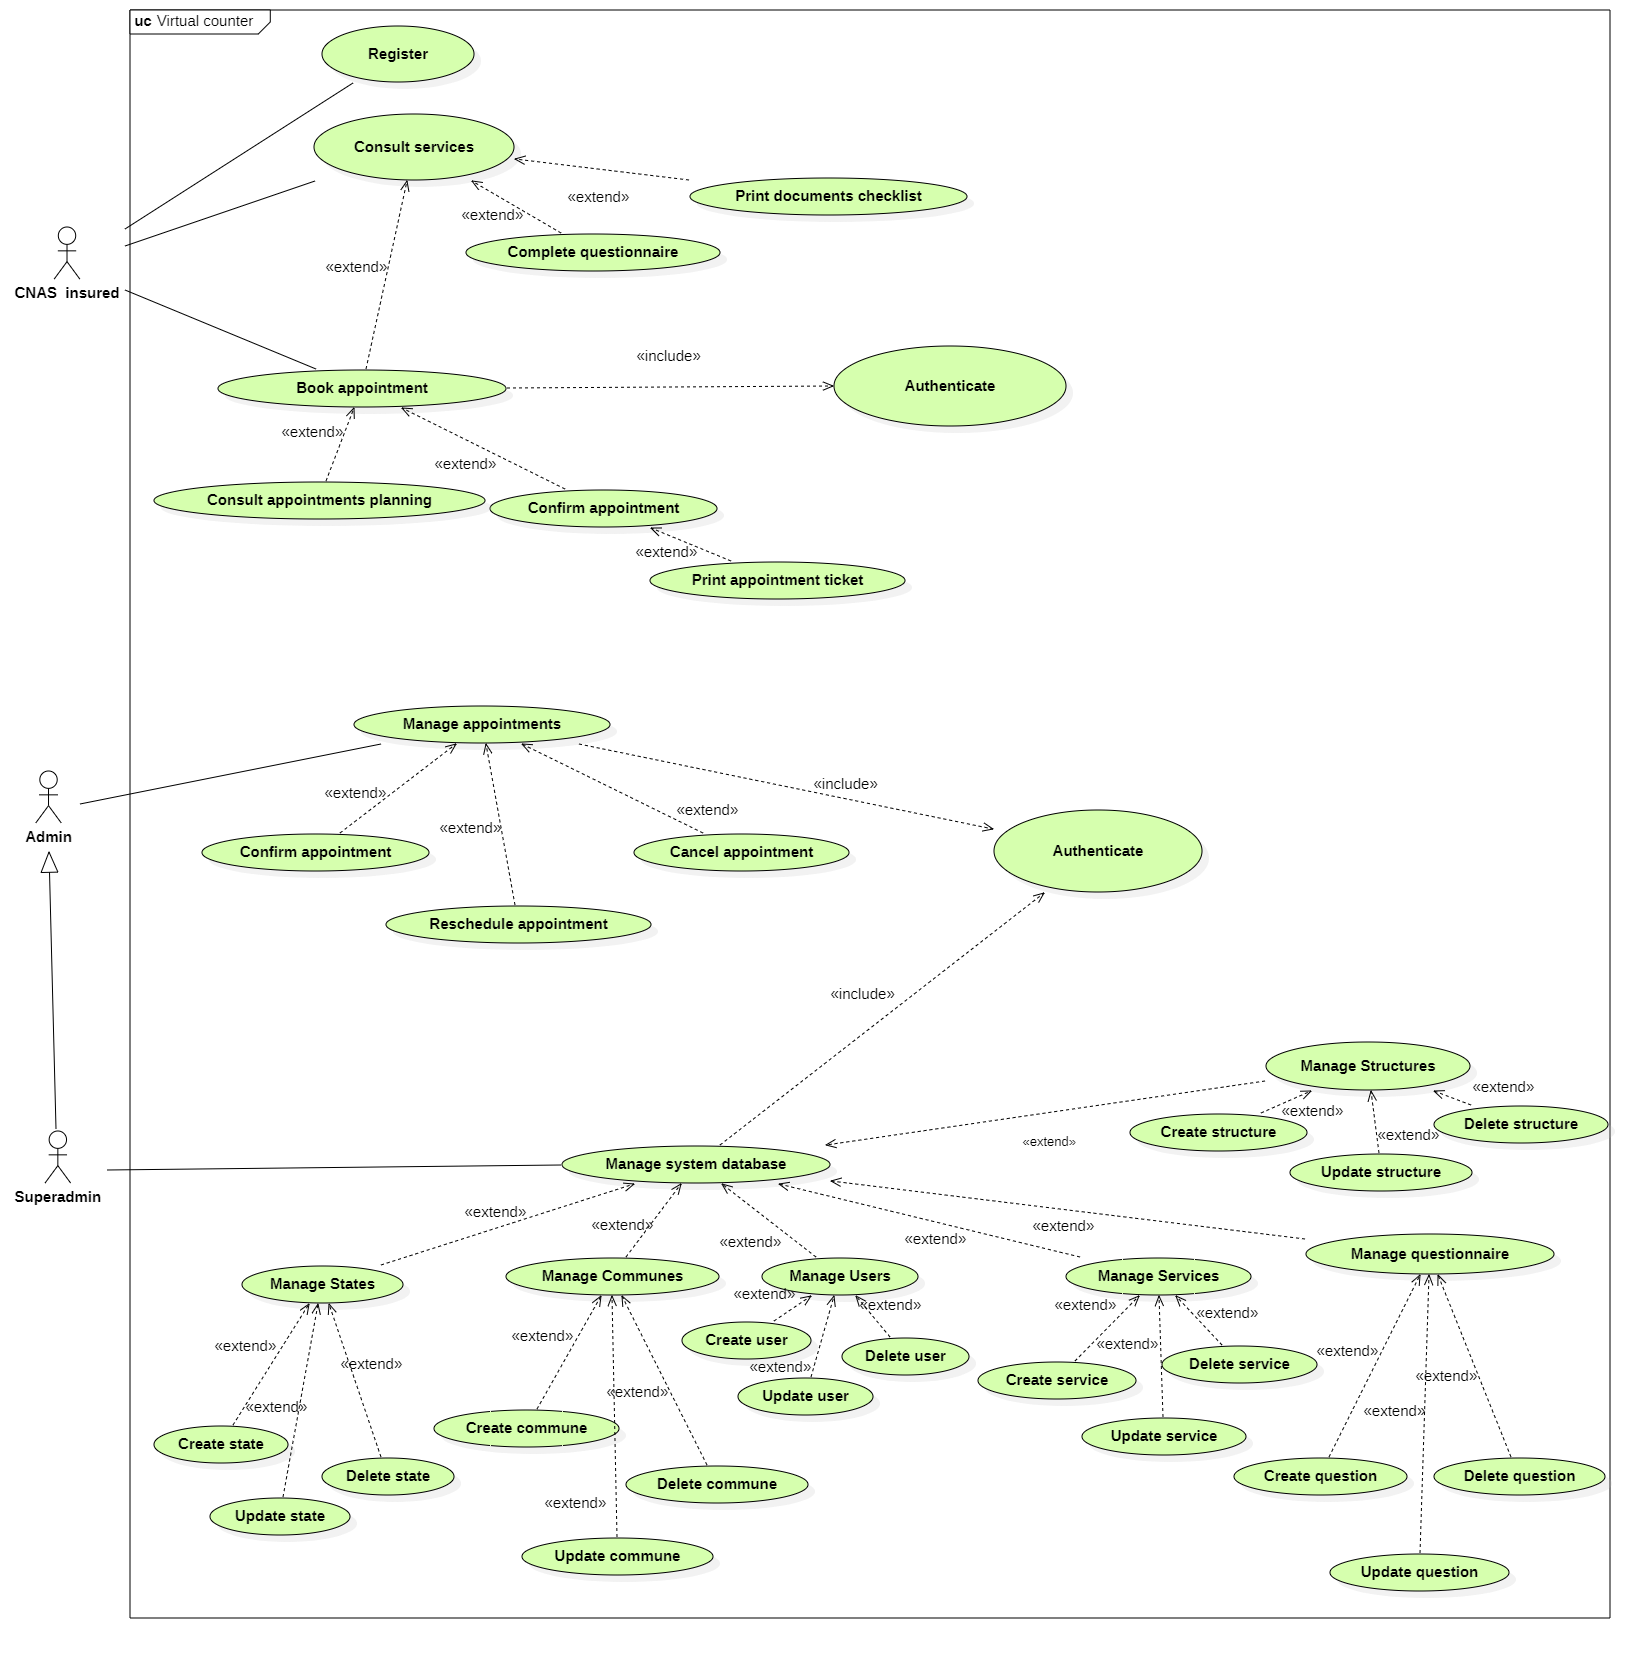
\includegraphics[width=1.0\textwidth]{UseCase.PNG}
    \caption{Use case diagram}
    \label{ucdiagram}
 \end{figure}
 
\subsection{Class diagram}
Class diagram is one of the static diagrams used to illustrate the overall architecture of the classes utilized in the application , it helps developers to capture the global planing of the project in which  will simplify the development in the first phases and the maintenance in the final product . 

\medskip On the same token , a collection of a class diagram represents the whole system . In addition the virtual counter conception we focused on tracing the whole activities of the user and the CNAS employee , so that it will be easy and much more efficient for the supervisor to track and see the statistics of the application . 

\begin{figure}[H]
    \centering
    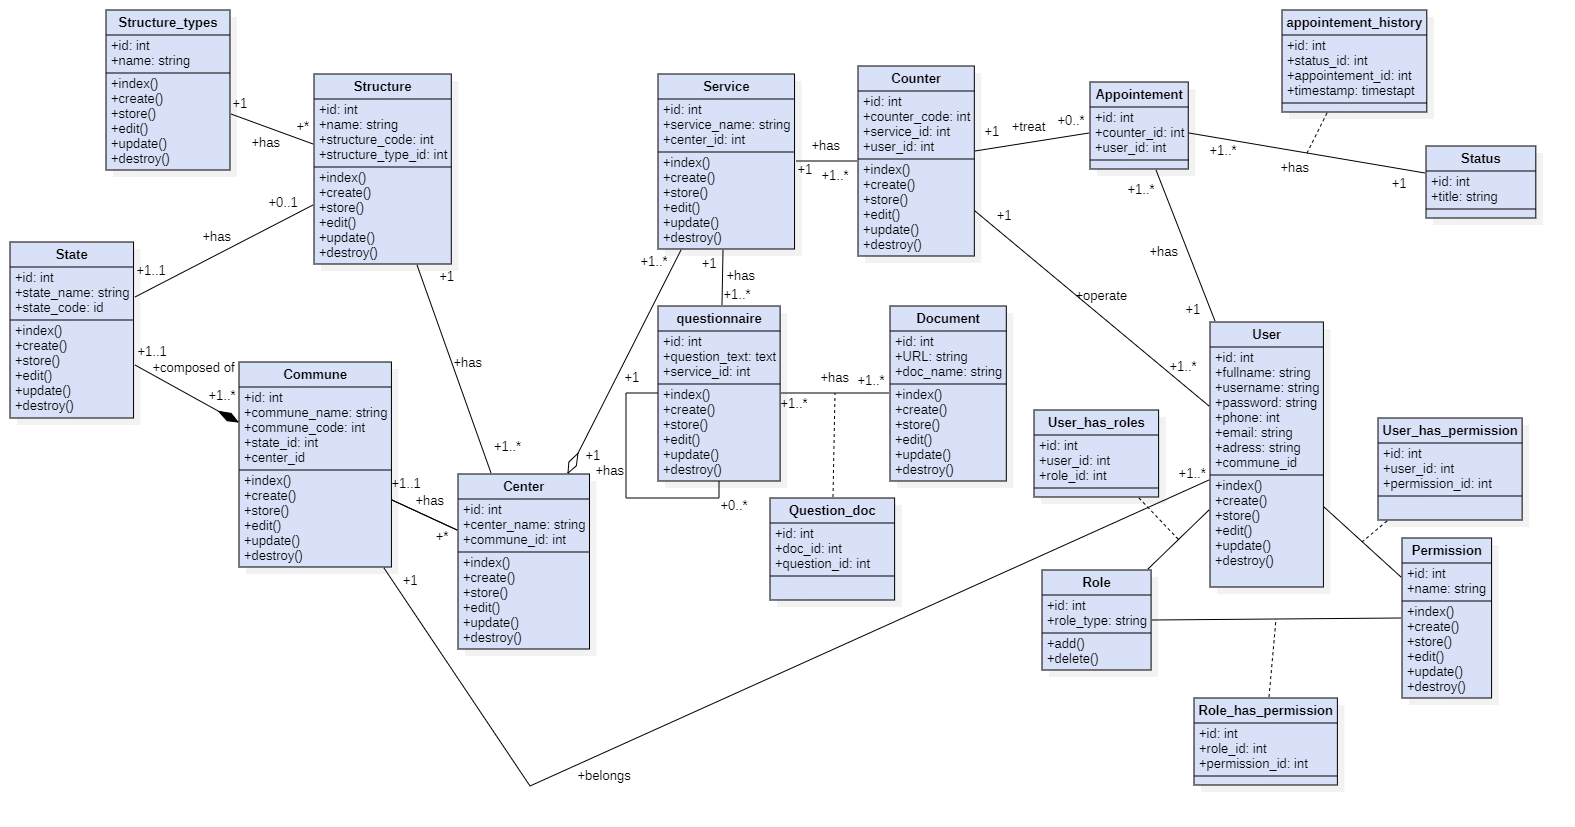
\includegraphics[width=1.0\textwidth]{ClassDiagram.png}
    \caption{Class diagram}
    \label{fig:Class diagram }
\end{figure}

\subsection{Sequence diagram}
Sequence diagram in one of the well known dynamic diagrams that allow the overall understanding for the hidden functionalities , and streamlines the developemnt phase . 

\medskip Here is the different diagrams related to every user in the application as well as the registration sytem . 
  \begin{figure}[H]
      \centering
      \includegraphics*[width=0.6\textwidth]{registration_sequence.PNG}
      \caption{Sequence diagram for Registration}
      \label{fig:Sequence diagram for Registration}
  \end{figure}
  \begin{figure}[H]
      \centering
      \includegraphics*[width=0.6\textwidth]{sequence_client.PNG}
      \caption{Sequence diagram for client interaction}
      \label{fig:Sequence diagram for Cient Interaction}
  \end{figure}
 
\subsection{Discussion of the design decisions made}
On the whole idea of  eliminating the wating time in such an efficient maner and to guarantee a powerful system , we reached to a finale conception of the virtual counter, which can assure by far a perfect user experience and a robust system in both sides as beneficiary or an employee . 

\medskip The use of this perticular system can be beneficial since we focused on creating a web application that covers all the problems that may be incontered along the working time of the application . 
 
For instence , if we consider that the patient want to get information it not recommended to force him to create an account since it's an information gathering , although booking an appointment in one of the services require the use of the patient information such as the name , adress ... ect , so it recommended to create an account that assures the integrity of his identity .    
\section{Database design}
In this juncture of the conception our main focus was on designing a reliable data base that can satisfy the needs of the virtual counter , along with offering the stakeholders the possibility to track and store the data efficiently and making sure that accessing the data will be in a secure process . 

//////
/////
\subsection{Overview of the database schema}
//
\subsection{Explanation of the different tables and their relationships}
//
\subsection{Discussion of the design decisions made}

//